\documentclass[11pt,a4paper]{article}
\usepackage[margin=2.2cm]{geometry}
\usepackage[T1]{fontenc}
\usepackage{lmodern}
\usepackage{xcolor}
\usepackage{tabularx}
\usepackage{booktabs}
\usepackage{enumitem}
\usepackage{titlesec}
\usepackage[hidelinks]{hyperref}
\usepackage{tcolorbox}
\usepackage{graphicx}

\definecolor{accent}{HTML}{1F4E79}
\definecolor{ok}{HTML}{2E7D32}
\definecolor{soft}{HTML}{EEF3F8}

\titleformat{\section}{\large\bfseries\color{accent}}{}{0pt}{}
\titlespacing*{\section}{0pt}{14pt}{6pt}
\setlist{itemsep=2pt,topsep=4pt}
\setlength{\parindent}{0pt}
\setlength{\parskip}{5pt}

\newcommand{\pass}{\textcolor{ok}{\textbf{Passed}}}
\newcommand{\cmd}[1]{\colorbox{soft}{\texttt{\small #1}}}

\begin{document}

{\LARGE\bfseries\color{accent} Gain PoC}\\[2pt]
{\large Audio plugin proof of concept}\\[2pt]
{\small\color{gray} October 2026 \quad\textbullet\quad \url{https://github.com/omverma1810/JUCE}}

\vspace{6pt}
\begin{tcolorbox}[colback=soft,colframe=accent,boxrule=0.6pt,arc=2pt]
\textbf{In one line:} we built a small volume-control plugin that loads and works in a
professional music app, proving we can deliver the client's real plugin.
\end{tcolorbox}

\section{What the client asked for}
The client has an idea for an audio plugin and wants a developer who can build it in the
three standard formats (\textbf{VST3}, \textbf{AU} and \textbf{AAX}). Before that, they asked for a
\emph{small proof of concept}: build a simple plugin, load it in \textbf{REAPER}, and check
it in \textbf{Logic Pro}.

The plugin itself is deliberately simple. The real test is whether we can take a plugin
from code all the way to something that works inside real music software.

\section{What we built}
\textbf{Gain PoC} is a single-knob volume plugin (from silent up to +12 dB).
\begin{itemize}
  \item \textbf{Three versions from one codebase:} VST3 (REAPER, Cubase, Ableton\dots),
        AU (Logic, GarageBand) and a standalone app.
  \item \textbf{Runs on every modern Mac:} both Apple Silicon and Intel.
  \item \textbf{Behaves like a professional plugin:} smooth volume changes with no clicks,
        the knob can be automated, and settings are saved with the project.
  \item \textbf{Built with JUCE 8}, the framework most commercial plugins are built on.
\end{itemize}

\section{How we know it works}
\begin{tabularx}{\linewidth}{@{}Xl@{}}
\toprule
\textbf{Check} & \textbf{Result} \\
\midrule
Apple's official plugin test (\texttt{auval}), Apple Silicon and Intel & \pass \\
Industry stress test (\texttt{pluginval}), strictest level, both formats & \pass \\
Loaded in REAPER 7.82 as VST3 and AU & \pass \\
Knob set to $-6$\,dB in REAPER $\rightarrow$ audio measured exactly 6\,dB quieter & \pass \\
\bottomrule
\end{tabularx}

\vspace{4pt}
All test reports and audio files are in the GitHub repository.

\section{Run it locally}
\textbf{You need:} a Mac with Xcode, Homebrew and REAPER (60-day free trial).
\begin{enumerate}
  \item Install the build tool:\\ \cmd{brew install cmake}
  \item Download the project:\\ \cmd{git clone -{}-recurse-submodules https://github.com/omverma1810/JUCE.git}
  \item Build it (the first build takes a few minutes):\\
        \cmd{cd JUCE} \\
        \cmd{cmake -B build -G Xcode} \\
        \cmd{cmake -{}-build build -{}-config Release}
  \item That's it. The plugin is installed automatically, and REAPER finds it on its next launch.
        The standalone app is in \texttt{build/GainPlugin\_artefacts/Release/Standalone/}.
\end{enumerate}

\section{How to demonstrate it (about 5 minutes)}
Screen-record this, with the system audio audible.
\begin{enumerate}
  \item \textbf{Show the project:} the GitHub page and the test results above.
  \item \textbf{Open REAPER:} drag any song or audio file onto a new track.
  \item \textbf{Add the plugin:} click the track's \textbf{FX} button and search for
        \emph{Gain PoC}. Pick the VST3 version.
  \item \textbf{Play and turn the knob:} the volume changes smoothly as you turn it.
  \item \textbf{Automate it:} show the track's envelopes, draw a volume curve for
        \emph{Gain} and play it back. The knob moves by itself.
  \item \textbf{Save and reopen:} save the project, close it and reopen it.
        The knob is where you left it.
  \item \textbf{Repeat with the AU version}, to show both formats work.
  \item \textbf{Optional:} open the standalone \emph{Gain PoC} app and play your
        microphone through it.
\end{enumerate}

\section{About Logic Pro}
Logic Pro is a paid app, but Apple offers a \textbf{free 90-day trial}. Two free alternatives:
\begin{itemize}
  \item \textbf{GarageBand} (free on the Mac App Store) uses the same audio engine as
        Logic. If the AU works in GarageBand, it will work in Logic.
  \item \textbf{JUCE AudioPluginHost}, a free test app we have already built, loads both versions.
\end{itemize}

\section{Next steps for the real plugin}
\begin{itemize}
  \item \textbf{Scope the client's idea:} effect or instrument, controls, and how the interface should look.
  \item \textbf{AAX (Pro Tools):} needs the client's Avid developer account and signing tools.
  \item \textbf{Distribution:} sign and notarize the plugin with Apple so it installs cleanly
        on any Mac, and package it as an installer.
  \item \textbf{Windows:} the same code can be built for Windows when needed.
\end{itemize}

\newpage
\section{Going further: Vibe FX}
To make the demo more impressive, we built a second plugin, \textbf{Vibe FX}: an effects rack with
the sounds people use in TikTok and YouTube song edits, plus a live dashboard.

\begin{center}
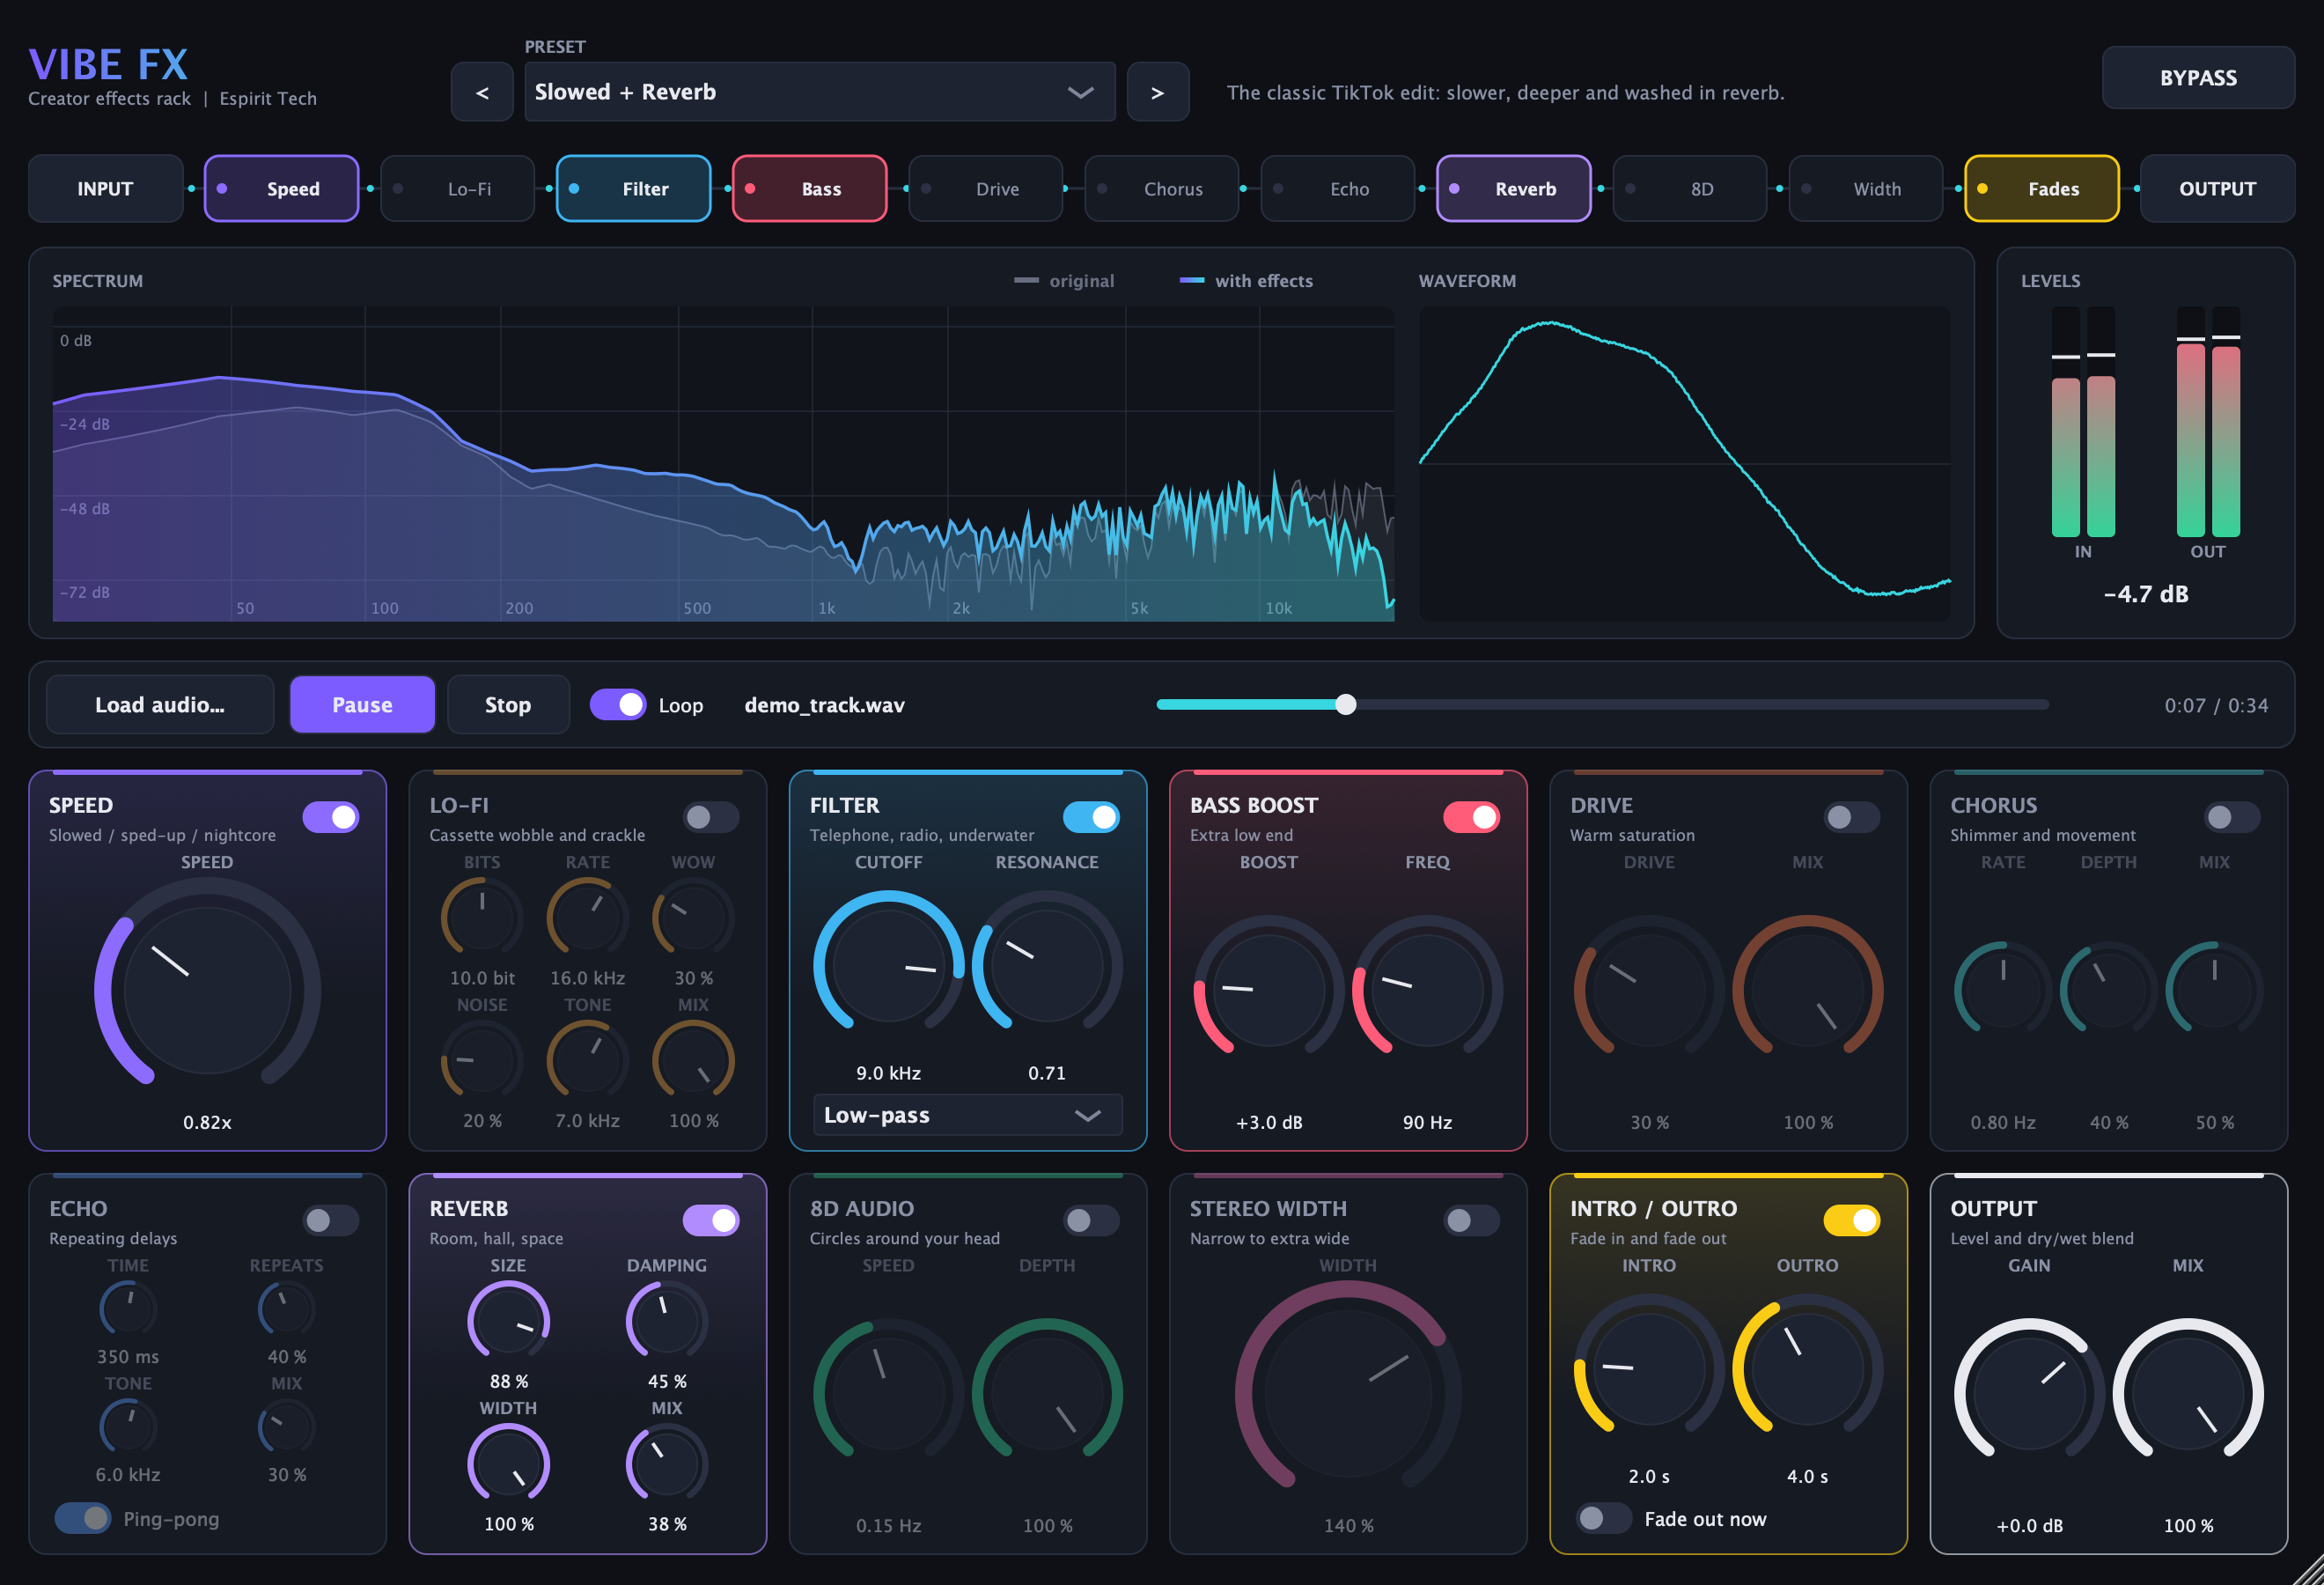
\includegraphics[width=\linewidth]{images/vibefx_slowed_reverb.png}
\end{center}

\begin{itemize}
  \item \textbf{11 effects:} speed (slowed / sped-up), lo-fi, filter, bass boost, drive, chorus,
        echo, reverb, 8D audio, stereo width, and intro/outro fades.
  \item \textbf{15 one-click presets:} Slowed + Reverb, Nightcore, Lo-Fi Chill, Vaporwave, 8D Audio,
        Telephone, Old Radio, Underwater, Echo Canyon, Bass Boosted and more.
  \item \textbf{Live dashboard:} see which effects are on, compare the original and processed sound
        on a spectrum display, and watch the waveform and levels.
  \item \textbf{Built-in player:} drop any song into the standalone app; no music software needed.
  \item \textbf{Tested:} passes Apple's official plugin test (auval), and all 15 presets
        were rendered in REAPER.
\end{itemize}

\textbf{Demo in 3 minutes:}
\begin{enumerate}
  \item Double-click \texttt{demo/Start Vibe FX Demo.command}: the app opens with a demo song loaded.
        (Or open \emph{Vibe FX} and drop any song onto it.)
  \item Press \textbf{Play}, then step through the presets with the \textbf{<} \textbf{>} buttons.
  \item Click \textbf{Bypass} to switch between the original and the effect.
  \item Turn a few knobs and watch the spectrum and signal chain react.
  \item In REAPER, open \texttt{demo/vibefx\_presets/VibeFX\_demo.rpp} to show it inside a DAW.
\end{enumerate}
Pre-rendered examples of every preset are in \texttt{demo/vibefx\_presets/}.

\end{document}
